%\clearpage
%\addcontentsline{toc}{chapter}{Appendices}
\begin{appendices}
\chapter{\label{appendix}}
\end{appendices}

\section{Comparison with the increasing number of layers}
How to select number of layers for the DNN model? With the fixed number of 512 nodes in each layer, the corresponding output comparison can be seen in \autoref{tab:app_1}

\begin{table}[H]
    \centering
    \begin{tabular}{c|c|c} \hline
      \# of Layers in the DNN  & Training Accuracy(\%) &  Testing Accuracy (\%)  \\ \hline \hline
      
       One(NN)        &     80.24   &    79.97  \\
       Two      &  82.15 & 81.59    \\
        Three    & 82.68 & 82.08  \\
        Four &  82.49 & 81.94 \\\hline \hline
    \end{tabular}
    \caption{Training and testing accuracy after training with simulated samples of Tprime(600-700GeV) with the standard model Higgs(SMH) backgrounds with each layer having 512 nodes.}
    \label{tab:app_1}
\end{table}






\subsection{One layer Only}
\begin{figure}[H]
     \centering
     \begin{subfigure}[b]{0.3\textwidth}
         \centering
         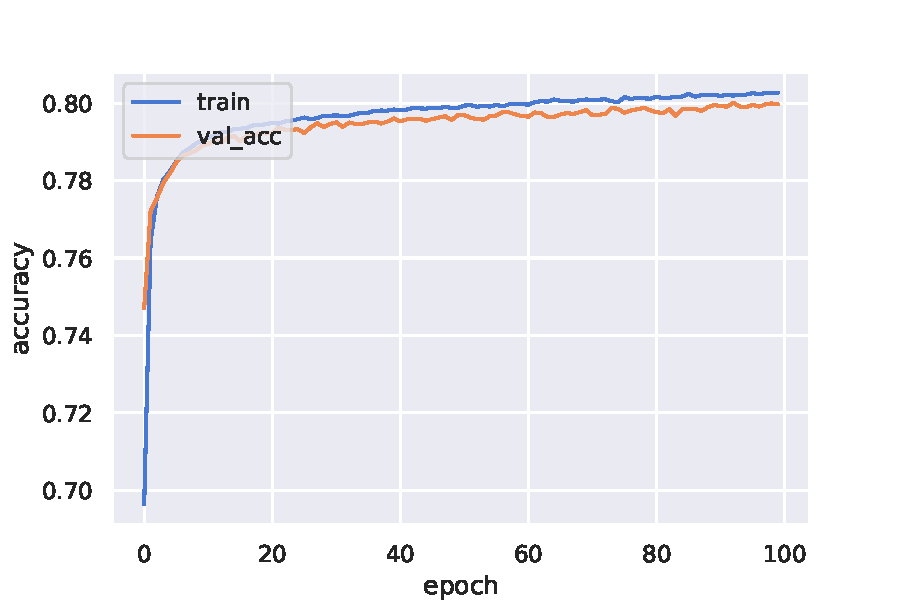
\includegraphics[width=\textwidth]{figure_3/One_node_only_accuracy.pdf}
         \caption{Model Accuracy}
         \label{fig:y equals x}
     \end{subfigure}
     \hfill
     \begin{subfigure}[b]{0.3\textwidth}
         \centering
         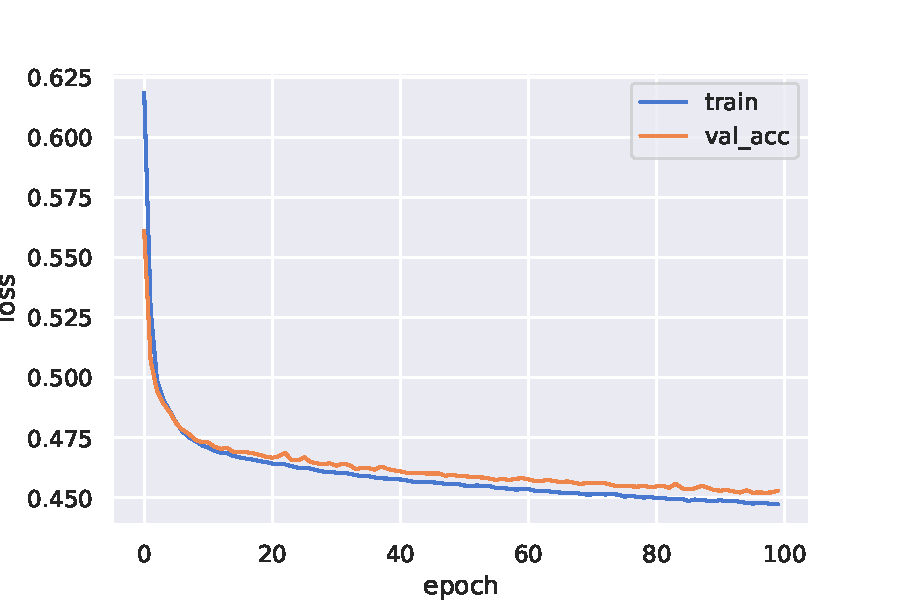
\includegraphics[width=\textwidth]{figure_3/One_node_only_loss.pdf}
         \caption{Model Loss}
         \label{fig:three sin x}
     \end{subfigure}
     \hfill
     \begin{subfigure}[b]{0.3\textwidth}
         \centering
         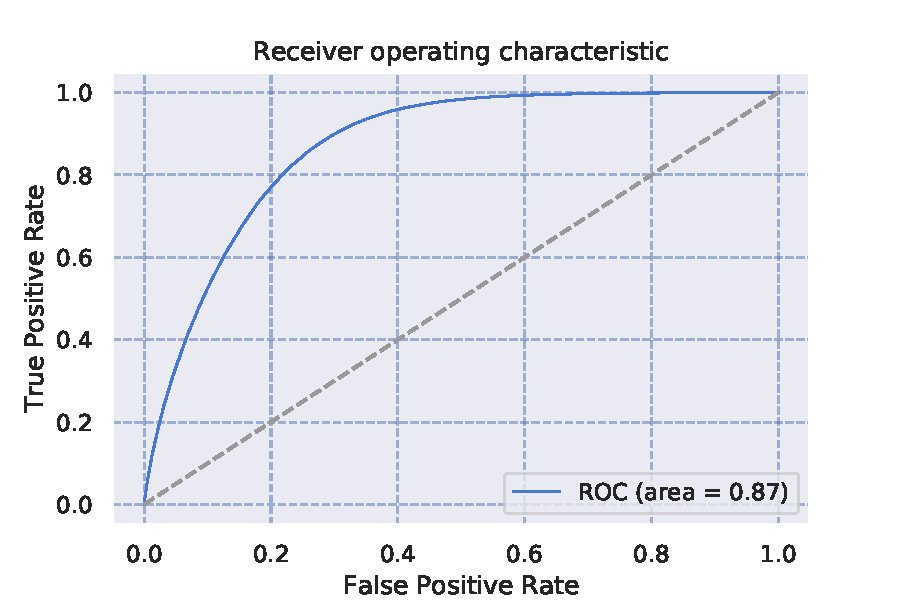
\includegraphics[width=\textwidth]{figure_3/one_layer_only_ROC.pdf}
         \caption{Model ROC Curve}
         \label{fig:five over x}
     \end{subfigure}
        \caption{Output corresponding to the training with only one layer(NN)}
        \label{fig:three graphs}
\end{figure}


\subsection{Two layers }
\begin{figure}[H]
     \centering
     \begin{subfigure}[b]{0.3\textwidth}
         \centering
         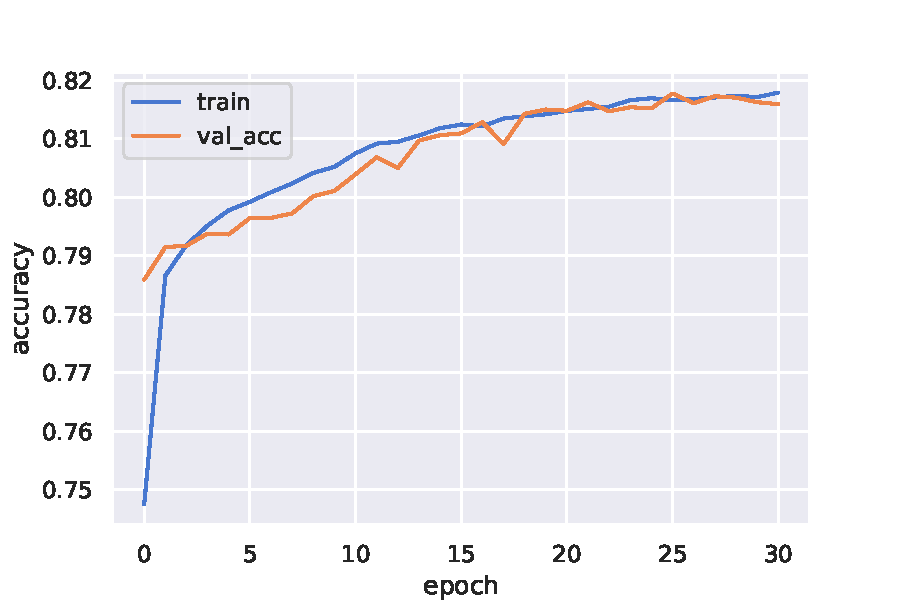
\includegraphics[width=\textwidth]{figure_3/One_node_two_accuracy.pdf}
         \caption{Model Accuracy}
         \label{fig:y equals x}
     \end{subfigure}
     \hfill
     \begin{subfigure}[b]{0.3\textwidth}
         \centering
         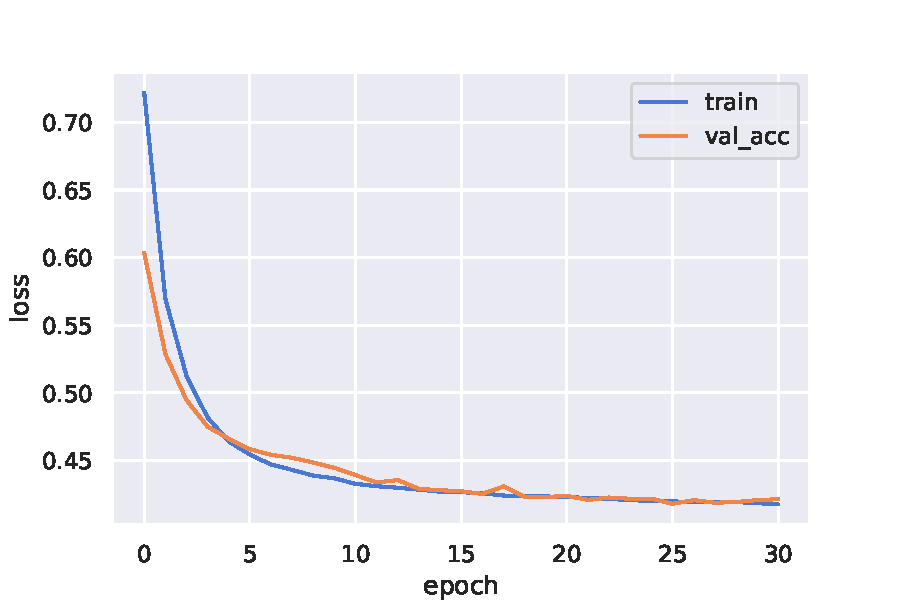
\includegraphics[width=\textwidth]{figure_3/One_node_two_loss.pdf}
         \caption{Model loss}
         \label{fig:three sin x}
     \end{subfigure}
     \hfill
     \begin{subfigure}[b]{0.3\textwidth}
         \centering
         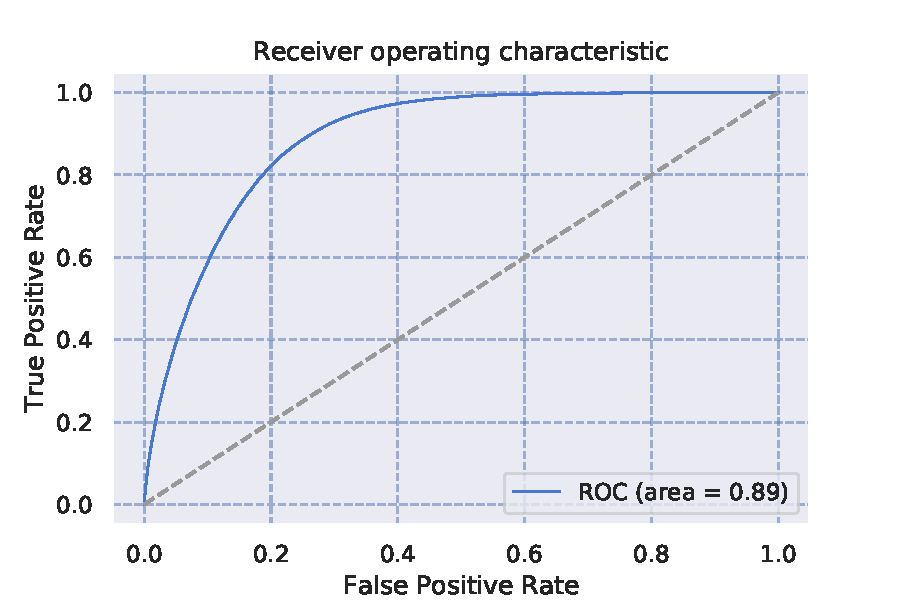
\includegraphics[width=\textwidth]{figure_3/two_layer_only_ROC.pdf}
         \caption{Model ROC Curve }
         \label{fig:five over x}
     \end{subfigure}
        \caption{Output corresponding to the training with two layers}
        \label{fig:three graphs}
\end{figure}


\subsection{Three layers}
\begin{figure}[H]
     \centering
     \begin{subfigure}[b]{0.3\textwidth}
         \centering
         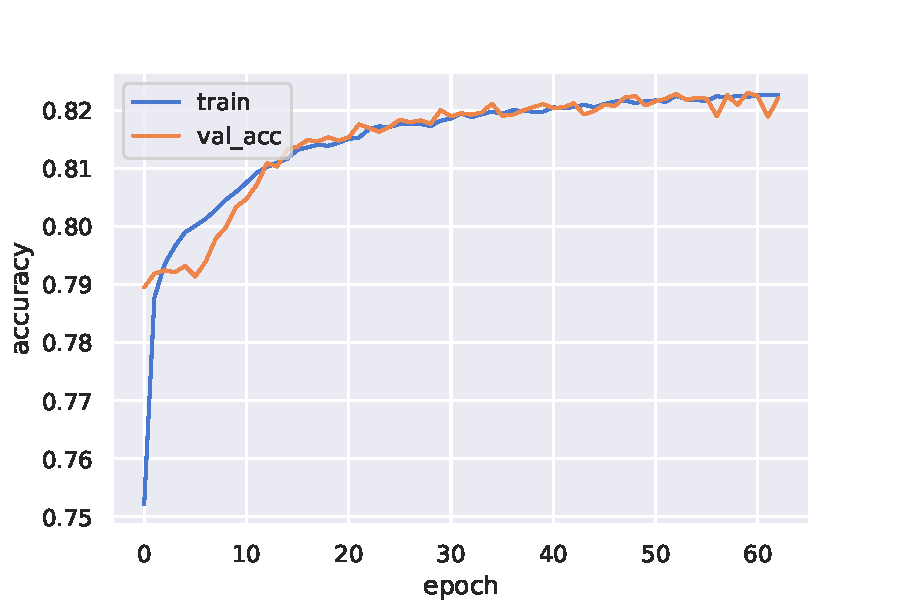
\includegraphics[width=\textwidth]{figure_3/One_node_three_accuracy.pdf}
         \caption{Model Accuracy}
         \label{fig:y equals x}
     \end{subfigure}
     \hfill
     \begin{subfigure}[b]{0.3\textwidth}
         \centering
         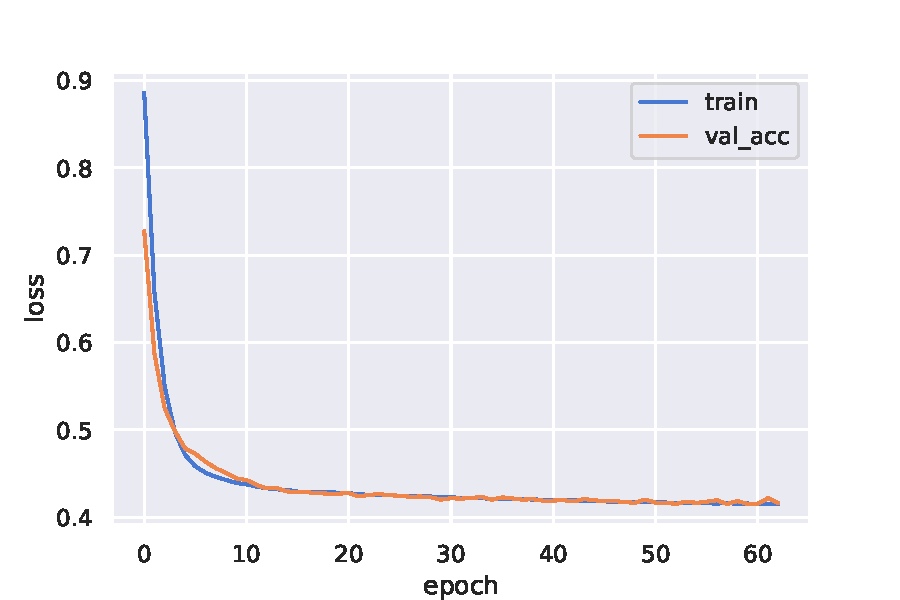
\includegraphics[width=\textwidth]{figure_3/One_node_three_loss.pdf}
         \caption{Model loss}
         \label{fig:three sin x}
     \end{subfigure}
     \hfill
     \begin{subfigure}[b]{0.3\textwidth}
         \centering
         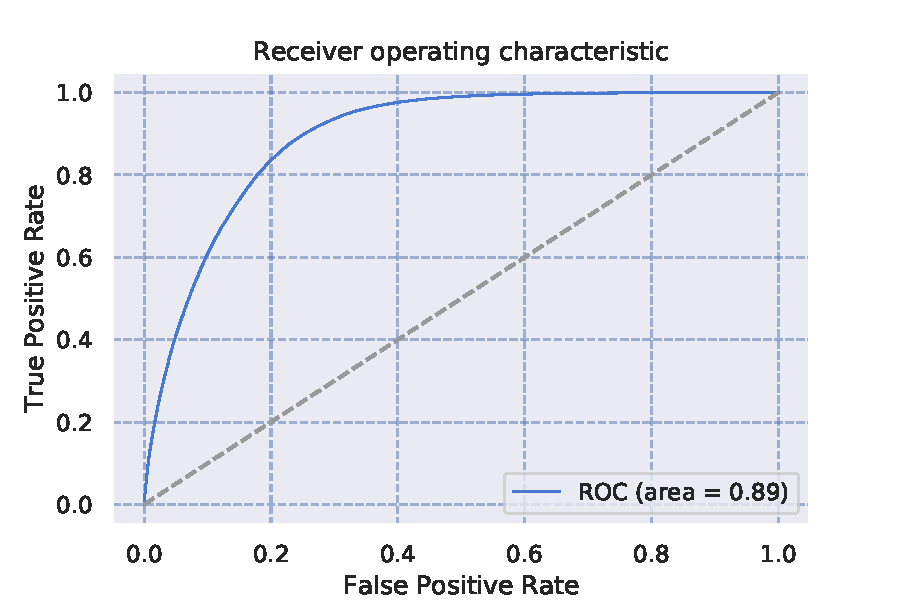
\includegraphics[width=\textwidth]{figure_3/three_layer_only_ROC.pdf}
         \caption{Model ROC Curve}
         \label{fig:five over x}
     \end{subfigure}
        \caption{Output corresponding to the training with three layers}
        \label{fig:three graphs}
\end{figure}




\subsection{Four layers}
\begin{figure}[H]
     \centering
     \begin{subfigure}[b]{0.3\textwidth}
         \centering
         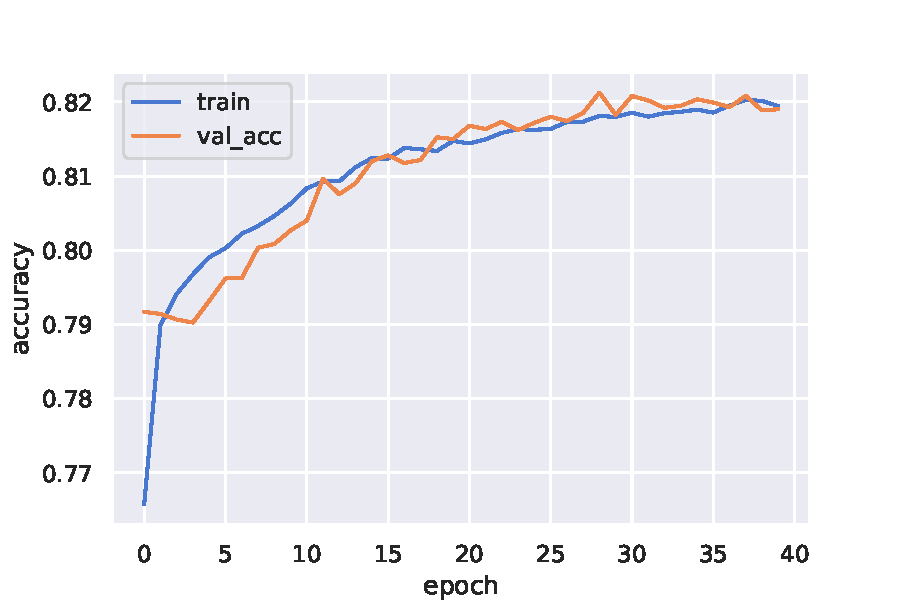
\includegraphics[width=\textwidth]{figure_3/One_node_four_accuracy.pdf}
         \caption{Model Accuracy}
         \label{fig:y equals x}
     \end{subfigure}
     \hfill
     \begin{subfigure}[b]{0.3\textwidth}
         \centering
         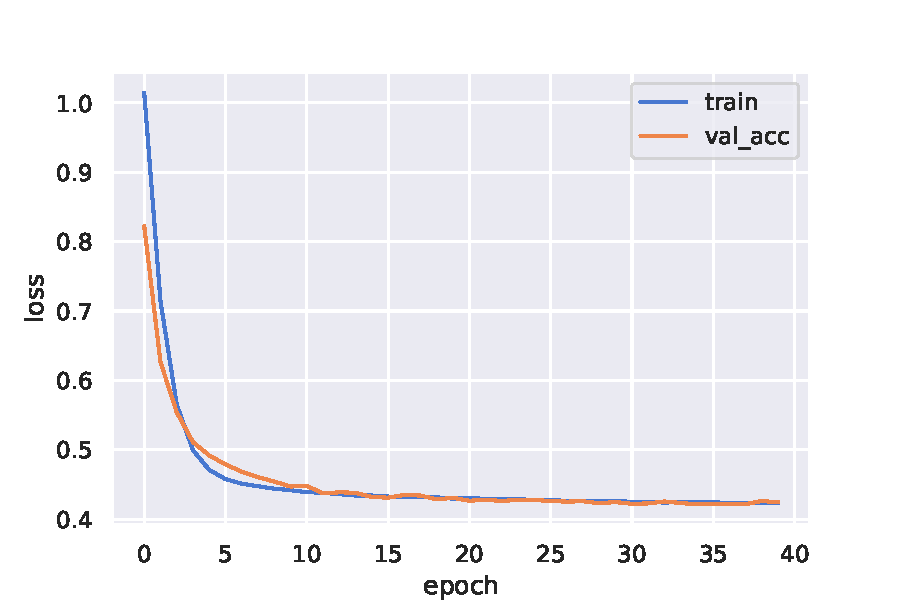
\includegraphics[width=\textwidth]{figure_3/One_node_four_loss.pdf}
         \caption{Model Loss}
         \label{fig:three sin x}
     \end{subfigure}
     \hfill
     \begin{subfigure}[b]{0.3\textwidth}
         \centering
         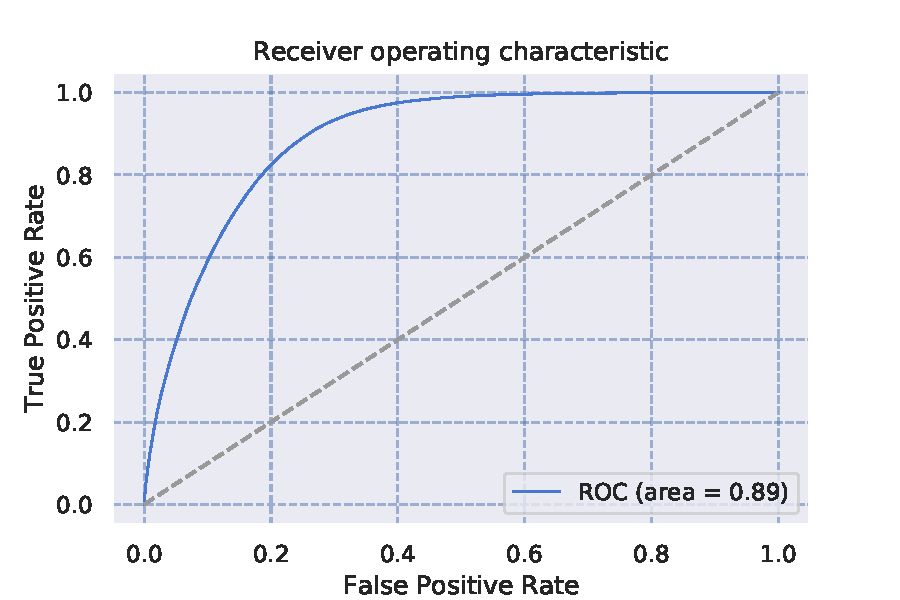
\includegraphics[width=\textwidth]{figure_3/four_layer_only_ROC.pdf}
         \caption{Model ROC Curve}
         \label{fig:five over x}
     \end{subfigure}
        \caption{Output corresponding to the training with four layers}
        \label{fig:three graphs}
\end{figure}





\subsubsection{Comparison of ROC}
\begin{figure}[h]
    \centering
    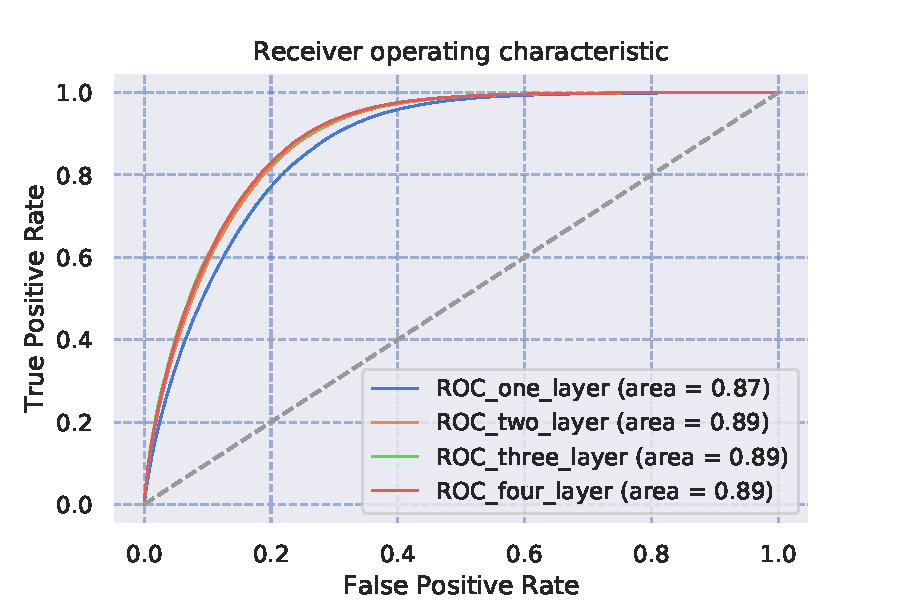
\includegraphics{figure_3/comaprision_ROC_with_layer_only_ROC.pdf}
    \caption{ROC comparison for different number of layers after keeping all other parameters for the DNN training constant. The ROC curve increases from single layer to two layer, while it get remains constant up to the four layers. On further increasing the number of layers, the model get overfit and the ROC-AUC decreases, which is also evident from \autoref{tab:app_1}}
    \label{fig:my_label}
\end{figure}



\setcounter{equation}{0}
\setcounter{table}{0}
\setcounter{figure}{0}
%\baselineskip 24pt


    



